\chapter{Сеанс работы в Linux}

\section{Задание}
	Определение понятий и анализ работы ниже названных объектов и процессов, которые происходят при сеансе работы в Linux:
\begin{itemize}
	\item Загрузка системы, ядро ​​системы, регистрация в системе, имя входящего пользователя.
	\item Персональный компьютер, многопользовательская операционная система, 					пользователи, администраторы, домашний каталог.
	\item Учетная запись UID, GID, полное имя, командная оболочка, интерпретатор командной 	строки, задачи администратора и его UID и GID.
	\item Хост, пароль, приглашение командной строки, идентификация.
	\item Виртуальные консоли их интерфейс, вызов виртуальных консолей и работа в них.
	\item Графические консоли.
	\item Имя пользователя, сеанс работы в системе, выходной поток данных, выход из 			системы.
\end{itemize}
\section{Основная часть}
	Обработка работы команд:
\begin{enumerate}
	\item Регистрация в системе.
	\begin{figure}[h]
		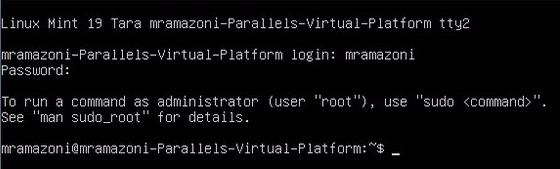
\includegraphics{lab1_2.png}
		\centering
	\end{figure}
	\newpage
	\item Изменение пароля.
	\begin{figure}[h]
		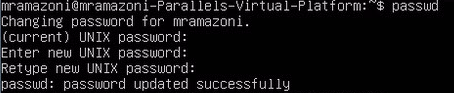
\includegraphics{lab1_3.png}
		\centering
	\end{figure}
	\item Определение учетной записи пользователя от имени которого выполняется работа.
	\begin{figure}[h]
		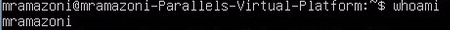
\includegraphics{lab1_4.png}
		\centering
	\end{figure}
	\item Вывод списка пользователей, которые в данный момент зарегистрированы в системе.
	\begin{figure}[h]
		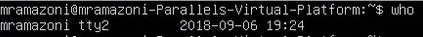
\includegraphics{lab1_5.png}
		\centering
	\end{figure}
	\item Вывод информации о пользователях, работавших в системе.
	\begin{figure}[h]
		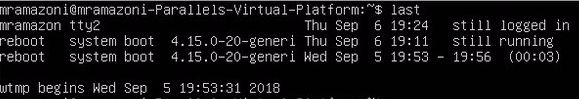
\includegraphics{lab1_6.png}
		\centering
	\end{figure}
	\item Выход из системы.
	\begin{figure}[h]
		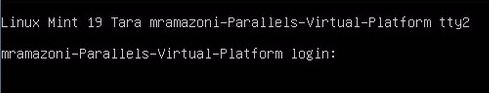
\includegraphics{lab1_1.png}
		\centering
	\end{figure}
\end{enumerate}

\section{Выводы}

